\section{Components of Training Neural Networks}

\subsection{MLPs are universal function approximators}

\begin{frame}\frametitle{\subsecname}


MLPs are universal function approximators. This means that, provided some assumptions are satisfied, they are capable of finding a function with which to map observations $\vec x$ to a their corresponding label $\vec y_T$.

   \begin{block}{The universal approximation theorem by Funahashi (1989)\footnote
	{ Funahashi (1989) On the approximate realization of 
		continuous mappings by neural networks. Neur Netw, 2:183--192\\
		Hornik et al. (1989) Multilayer Feedforward Networks 
		are Universal Approximators. Neur Netw, 2:359--366. }}
	\small
    	Let $y_T{(\vec{x})}$ be a continuous, real valued function 
    	over a compact interval $K$ and     
		\begin{equation} 
		{y}{(\vec{x}; \vec w)} = \sum_{i=1}^M \mathrm{w}_i^{21} 
		f\Big( \sum\limits_{j=1}^N \mathrm{w}_{ij}^{10} 
		  \mathrm{x}_j - \theta_i \Big)
		 \end{equation}
    	be a three-layered MLP with a non-constant, bounded, 
    	monotonously increasing and continuous function 
    	$f: \mathbb{R} \rightarrow \mathbb{R}$.\\
		\vspace{4mm}
	   \pause

		Then there exists a set of parameters 
		$M, N \in \mathbb{N}$ and $\mathrm{w}_i^{21}, 
		\mathrm{w}_{ij}^{10}, \theta_i \in \mathbb{R}$ 
		such that for every $\varepsilon > 0$:
		\begin{equation}
		\max_{\vec{x} \in K} \Big| \,{y}{(\vec{x}; \vec w)} - y_T{(\vec{x})} \,\Big| 
		\leq \varepsilon
		 \end{equation}
  \end{block}
  
\end{frame}

\subsection{Ingredients for function fitting}

\begin{frame}\frametitle{\subsecname}


Fit an MLP to desired function $y_T(\vec x)$ requires the following ingredients:

\begin{enumerate}
\item A cost function with the objective to minimize it: $e(y_T, \vec x)$.
\item A performance measure. Specifically, \\

the generalization error $E^G$ which is defined as:	
\begin{equation} 
			E^G \quad := \quad \left<\,e\,\right>_{y_T, \vec{x}} 
			\quad = \quad \iint d \vec{x} \, dy_T \; 
				P_{(y_T, \vec{x})} \, e_{(y_T, \vec{x})}
\end{equation}

\item A parameterized model: MLP, connecitonist neuron, \ldots
\item An optimization method or learning algorithm for finding the set of parameters in our model that will minimize the cost function.\\
This can be done analytically (depending on the conditions) or through an iterative learning algorithm (e.g. gradient-based learning)
\end{enumerate}

\end{frame}

\subsection{Cost functions}
\begin{frame}\frametitle{\subsecname}

A cost function $e(y_T, \vec x)$ (or more explicitly $e(y_T, y(\vec x; \vec w)$) quanitfies the discrepancy between the model's prediction for a specific observation and the label it is assigned to.

Selecting a cost function accounts for 
\begin{enumerate}
\item the type of problem (i.e. regression vs. classification) and 
\item how the model is penalized for different types of mistakes it can make such as:
tolerance for certain error range (e.g. small errors are tolerable), large errors are penalized less.
\end{enumerate}

The choice of cost function has a direct effect on how the model will learn. For example, we will later see in gradient-based learning how the error function can modulate how fast or slow  a model learns.

\end{frame}


\subsubsection{Cost functions for Regression}

\begin{frame}\frametitle{\subsecname}


  \begin{tabular}{c c c}
    \parbox{4cm}{
      \[ \underbrace{\vec{x}
          \in \mathbb{R}^N
      }_{\text{feature vector}}
      \longrightarrow 
      \underbrace{y
      \in \mathbb{R}
      }_{\text{attribute}}
      \]}
    & & 
    \parbox{8cm}{\footnotesize
      \begin{tabular}{l l}
	$y_T$: & true value of attribute \\
	$y(\vec{x})$: & predicted value of attribute (e.g. by MLP)
      \end{tabular}
    }
  \end{tabular}
     \pause

  \begin{block}{individual cost $e(y_T, \vec{x})$}
    \begin{center} 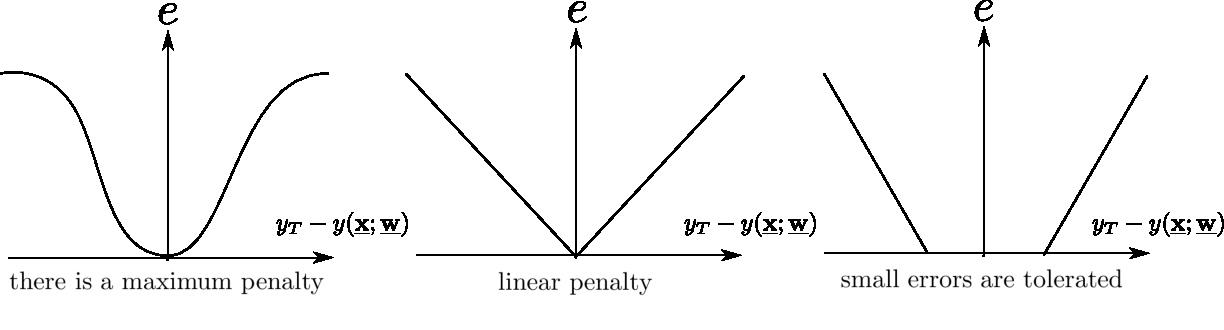
\includegraphics[width=12cm]{img/section1_fig17_v2.pdf} \end{center}
  \end{block}   %\pause
  \textbf{several choices $\Rightarrow$  predictor will depend on error measure!}

\end{frame}
